\documentclass[letterpaper,12pt,fleqn]{article}
\usepackage{matharticle}
\pagestyle{empty}
\newcommand{\n}{\mathrel{\triangleleft}}
\newcommand{\p}{\phi}
\begin{document}
\section*{Normal Subgroups}

\begin{definition}
  Let $H\le G$. To say that $H$ is a \emph{normal} subgroup of G,
  denoted $H\n G$, means:
  \[\forall\,g\in G,h\in H,ghg^{-1}\in H\]
\end{definition}

\begin{theorem}
  Let $\p:G\to G'$ be a homomorphism of groups and $K=\ker(\p)$:
  \[K\n G\]
\end{theorem}

\begin{theproof}
  Assume $g\in G$ and $k\in K$ \\
  $\p(gkg^{-1})=\p(gg^{-1})=\p(e)=e'$ \\
  $\therefore gkg^{-1}\in K$
\end{theproof}

\begin{theorem}
  Let $H\le G$. TFAE:
  \begin{enumerate}
  \item $H\n G$
  \item $\forall\,g\in G,gHg^{-1}=H$
  \item $\forall\,g\in G,gH=Hg$
  \end{enumerate}
\end{theorem}

\begin{theproof}
  Assume $g\in G$
  
  \begin{description}
  \item{$1\implies2$}: Assume $H\n G$

    \begin{minipage}[t]{3in}
      Assume $a\in gHg^{-1}$ \\
      $\exists\,h\in H,a=ghg^{-1}\in H$ \\
      $\therefore a\in H$
    \end{minipage}
    \begin{minipage}[t]{3in}
      Assume $a\in H$ \\
      $\exists\,h\in H,h=gag^{-1}$ \\
      $a=g^{-1}hg=g^{-1}h(g^{-1})^{-1}$ \\
      $\therefore a\in gHg^{-1}$
    \end{minipage}

  \item{$2\implies3$}: Assume $gHg^{-1}=H$

    \begin{minipage}[t]{3in}
      Assume $g'\in gH$ \\
      $\exists\,h'\in H,g'=gh'$ \\
      $gh'g^{-1}\in H$ \\
      $\exists\,h\in H,gh'g^{-1}=h$ \\
      $gh'=hg$ \\
      $g'=hg$ \\
      $\therefore g'\in Hg$
    \end{minipage}
    \begin{minipage}[t]{3in}
      Assume $g'\in Hg$ \\
      $\exists\,h'\in H,g'=h'g$ \\
      $g^{-1}h'g\in H$ \\
      $\exists\,h\in H,g^{-1}h'g=h$ \\
      $h'g=gh$ \\
      $g'=gh$ \\
      $\therefore g'\in gH$
    \end{minipage}
\newpage
  \item{$3\implies1$}: Assume $gH=Hg$

    $\forall\,h\in H,\exists\,h'\in H,gh=h'g$ \\
    $ghg^{-1}=h'$ \\
    $ghg^{-1}\in H$ \\
    $\therefore H\n G$
  \end{description}
\end{theproof}

\begin{corollary}
  Let $H\le G$:
  \[G\ \mbox{abelian}\implies H\n G\]
\end{corollary}

\begin{theproof}
  Assume $g\in G$ \\
  Assume $h\in H$ \\
  $ghg^{-1}=gg^{-1}h=eh=h$ \\
  $ghg^{-1}\in H$ \\
  $\therefore H\n G$
\end{theproof}

\begin{theorem}
  Let $H\le G$:
  \[(G:H)=2\implies H\n G\]
\end{theorem}

\begin{theproof}
  \begin{minipage}{3.5in}
    Assume $(G:H)=2$ \\
    Assume $a\in G,a\notin H$ \\
    $H$ and $aH$ are the two distinct left cosets \\
    $H$ and $Ha$ are the two distinct right cosets \\
    $aH=Ha$ \\
    $\therefore H\n G$
  \end{minipage}
  \begin{minipage}{3in}
    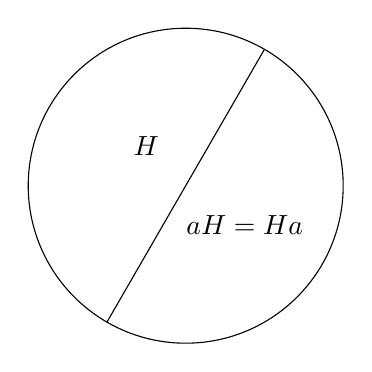
\begin{tikzpicture}
      \draw (0,0) circle [radius=2];
      \draw (-1,{-sqrt(3)}) -- (1,{sqrt(3)});
      \node at (-0.5,0.5) {$H$};
      \node at (0.75,-0.5) {$aH=Ha$};
    \end{tikzpicture}
  \end{minipage}
\end{theproof}

\begin{example}
  $(S_4:A_4)=2$

  $A_4$ elements are even \\
  $(12)A_4$ elements are odd \\
  $(12)A_4$=$A_4(12)$ \\
  $A_4\n S_4$
\end{example}

\end{document}
